In order to further optimize the code some profiling is needed to identify the bottleneck and solve them... If possible. \\
The methodology followed is to use \textbf{Intel VTune} on the entire regression. Profiling only the nnls portion of the code did not give reliable results because terminates too fast. Profiling the entire regression instead, gave interesting results; As showed in \ref{img:vtune_eigen_01} and \ref{img:vtune_eigen_02} there are two hotspots in the code. \\
\begin{figure}[ht]
  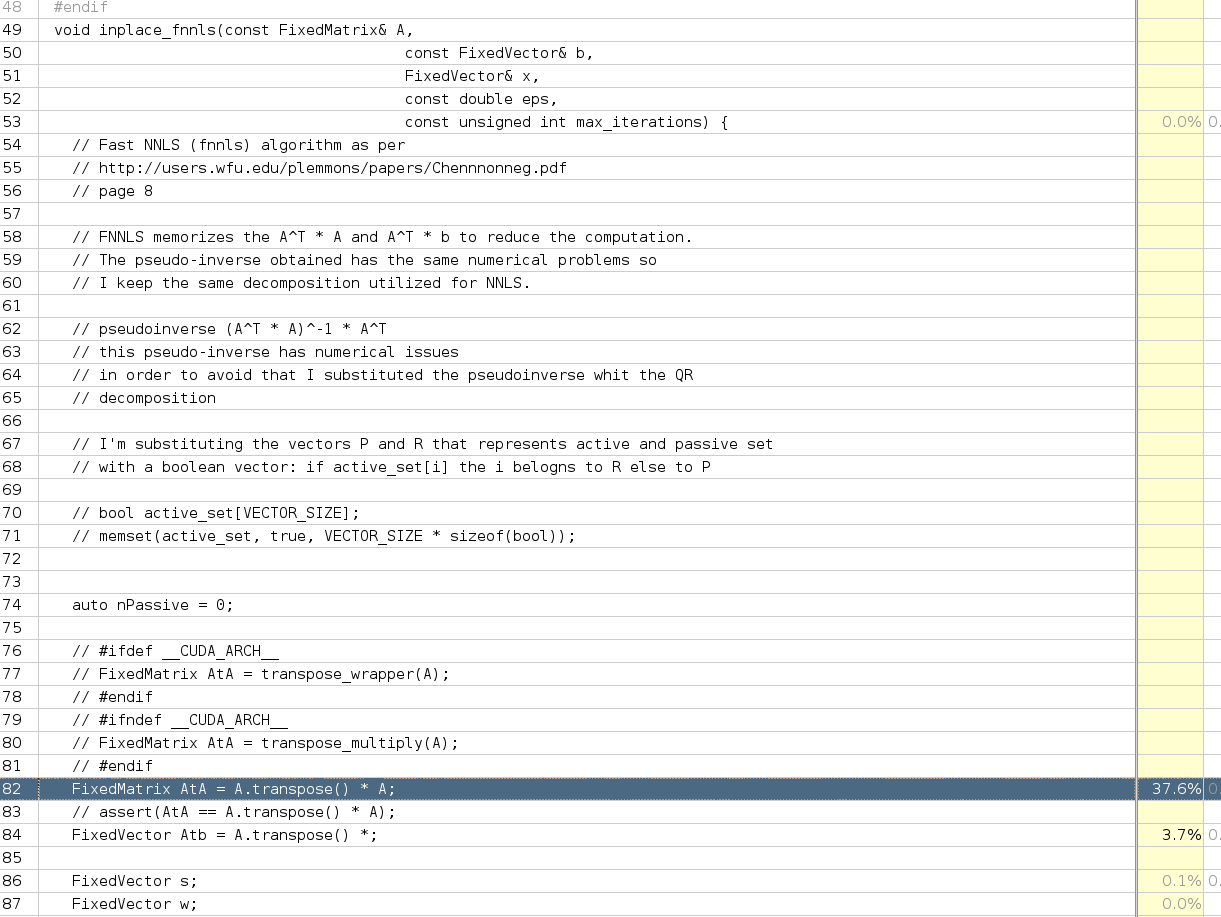
\includegraphics[width=\textwidth]{img/vtune_eigen_01}
  \caption{VTune profiling of multifit\_cpu. 37\% of the total time is spent performing $A^TA$.}
  \label{img:vtune_eigen_01}
\end{figure}
\begin{figure}[ht]
  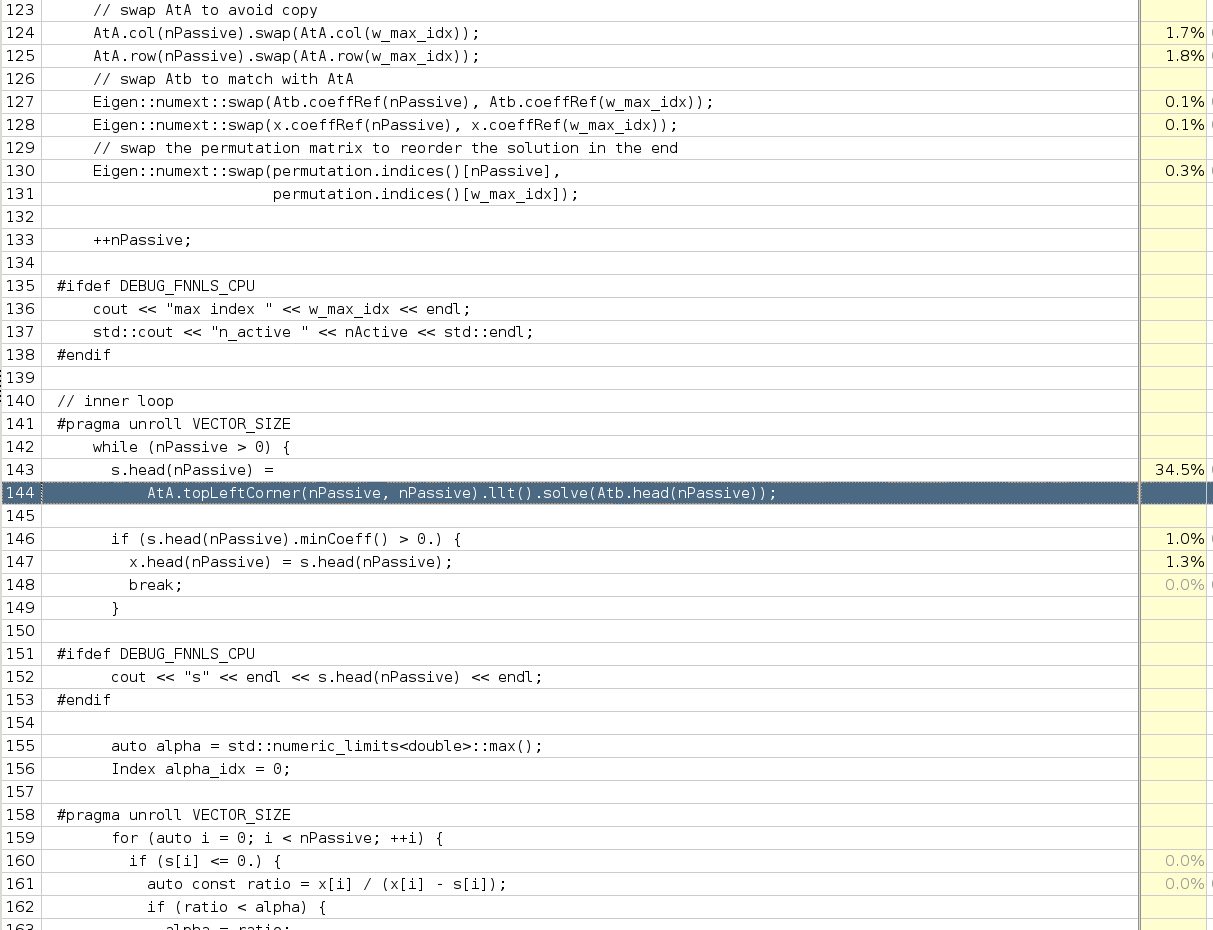
\includegraphics[width=\textwidth]{img/vtune_eigen_02}
  \caption{Second bottleneck found using VTune. 34\% of the time is spent calculating the Cholesky decomposition.}
  \label{img:vtune_eigen_02}
\end{figure}
The first hotspot is the computation of $A^TA$ that requires 37\% of the total execution time. To solve this hotspot it is possible by exploiting the observations:
\begin{itemize}
    \item The matrix $A^TA$ is symmetric so it is enough calculate the lower triangular portion and the copy the results back.
    \item The matrix is $10 \times 10$, it fits in L1 cache, thus cache efficiency is more important than algorithmic complexity.
\end{itemize}
Under this hypothesis is it possible to improve the eigen implementation to squeeze a little bit more performance out of it. \\
On the GPU side instead, is it possible to parallelize this product with a kernel invocation. \\
The second bottleneck can be solved using the closed formula present in \cite{wiki:Cholesky_decomposition} to update the Cholesky without recomputing it in case of adding/removing one column and one row.
